\documentclass[11pt,a4paper,english]{uvamath}
\usepackage[english]{babel}

\usepackage{amsmath, amsfonts, amssymb, a4wide, fancyhdr, lineno, graphicx, epsfig, soul, color, hyperref}
\usepackage[square, numbers]{natbib}

% Running line numbers:
\linenumbers
% Number only every 5:th line:
\modulolinenumbers[5]

%Nodig om een bibliography midden in het artikel te zetten, ipv aan het einde zoals eigenlijk gebruikelijk is
\renewcommand{\bibsection}{}

% TODO command
\newcommand{\todo}[1]{
    \hl{#1}
}

% The things that should be filled in by each group, depending on their situation, are written in a todo command, \todo{like this text}. All text in normal the normal font, is applicable for any group. However, everyone is free to adapt any text, and it is even suggested to look at all text critically and make changes if needed.

% Project specific commands
\author{Tom van Duist \& Kevin van den Bekerom}

\newcommand{\projectname}{\todo{Project Name}\ }


\newcommand{\aanpassen}[1]{ {\sethlcolor{green} \hl{#1}} }

\title{Requirements Document}
%Variables
\newcommand{\TitelAbbr}{RD}
\newcommand{\Version}{0.1}



\what{Lab assignment Requirements Engineering}
\supervisors{}

\coverimage{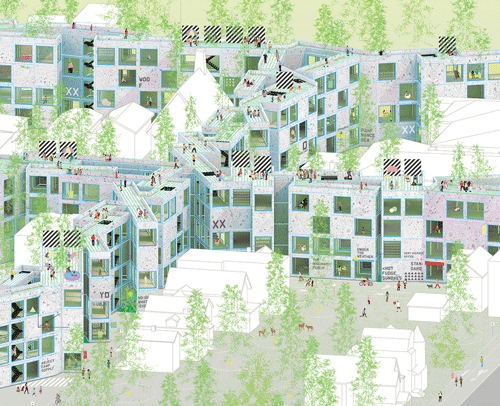
\includegraphics[scale=0.5]{Images/titleImage}\\
"\emph{The architecture giveth and the implementation taketh away.}"\\ - Len Bass, Paul Clements, Rick Kazman}


\begin{document}

\maketitle


\tableofcontents

\chapter*{Document Status Sheet}
\section*{Document status overview}
\subsection*{General}
\begin{tabular}[!]{ll}
    Document title:     & Architectural Design Document\\
    Authors:           	& Kevin van den Bekerom \\ 
						& Tom van Duist \\
    Document status:    & Draft release\\
\end{tabular}

\subsection*{Document history}
\begin{tabular}[!]{|l|l|l|l|}
    \hline
    \emph{Version}    &   \emph{Date} &  \emph{Reason of change}\\
    \hline
    0.0 & 02-09-2015 &  Setup of the document layout\\    
    \hline
    0.1 & 29-10-2015 & Release version week 1 \\
    \hline
\end{tabular}

\clearpage

%\section*{Document Change Records since previous issue}
%\subsection*{General}
%\begin{tabular}[!]{ll}
%   Datum:          &   2015-06-09 \\
%    Document title: &   Architectural Design Document (ADD)\\
%    Identification:  &   \TitelAbbr\_\Version.pdf\\
%\end{tabular}

%\subsection*{Changes}
%\begin{tabular}[!]{|l|l|p{8 cm}|}
%    \hline
%    \emph{Chapter} &   \emph{Paragraph}    &   \emph{Reason to change}\\
%    \hline
%    \ref{c:main_fun} &  whole chapter      & Make prioritizing clear using Moscov model. Clarified functionalities. \\
%    \hline
%    dfdf& tt & ff. \\
%    \hline
%\end{tabular} 

\chapter{Introduction}



\chapter{References}

\begin{thebibliography}{9}
	
	\bibitem{bosch}
	Jan Bosch,
	\emph{Software Architecture: The Next Step},
	University of Groningen, Department of Computing Science
	
	
	
\end{thebibliography}


\appendix


\end{document}
